\section{Experimental results}
\label{results}
\subsection{Datasets and evaluation protocol}
\label{subsec:datasets}
We use four public datasets \cite{kuehne2011, marszalek2009, niebles2010, reddy2013} and their corresponding evaluation protocols. In this section we briefly describe each dataset.

\textbf{HMDB51} \cite{kuehne2011} includes a large collection of human activities categorized on 51 classes. It collects 6766 videos from different media resources \ie digitized movies, public databases and user generated web video data. Due to a large amount of videos contains undesired camera motions, the authors provide a stabilized version of the dataset. However, since we look at the camera motion as an informative cue, non-stabilized version of the dataset is used. For evaluating performance, we adopt the same protocol proposed by the dataset authors \ie computing the mean accuracy under three fixed train/test splits.

\textbf{Hollywood2} \cite{marszalek2009} contains a wide number of videos retrieved from 69 different Hollywood movies. It is divided in 12 categories including short actions such as Kiss, Answer Phone and Stand Up. This dataset remains as one of the most challenging despite the small number of action classes. Change of camera view,  camera motion and unchoreographed execution introduces more difficult a the time of recognition. To evaluate performance, we follow the author's protocol where videos are separated in two different sets: a training set of 823 videos and a testing set of 884 videos. We use training videos to learn our action models and then compute the mean average precision (mAP) over all action classes.

\textbf{Olympic Sports} \cite{niebles2010} or \textbf\textit{{Olympic}} comprises a set of 783 sport related YouTube videos. This set of videos are semi-automatically labeled using Amazon Mechanical Turk. This dataset establish new challenges for recognition because of it jumps from simple actions (\eg Kiss) to complex actions (\eg Hammer throw). All of these complex actions are related with olympic sports including actions like \textit{Long jump}, \textit{Pole vault} and \textit{Javelin throw}. As proposed by the author's dataset, we measure performance calculating the mAP over all dataset categories.

\textbf{UCF50} \cite{reddy2013} includes 6618 videos of 50 different human actions.  This dataset presents several recognition challenges due to large variations in camera motion, cluttered background, viewpoint, etc. Action categories are grouped into 25 sets, where each set consists of more than 4 action clips. Recognition performance is measured by applying a leave-one-group-out cross-validation and average accuracy over all group splits is reported. 

\subsection{Implementation details}

\textbf{Visual descriptors}. Our better understanding of actions splits visual descriptors in two different groups. Next, we briefly give a detailed explanation of how these descriptors are extracted.
(a) \textbf{Foreground descriptors} \ie Trajectory Shape, HOG, HOF, and MBH are computed over dense trajectories using a modified implementation on \cite{wang2013}. To find inliers matches for compensating camera motion, we employ a Fundamental Matrix instead of computing a Homography. In the following, these foreground descriptors are computed with the same parameters as in \cite{wang2013}.
(b) \textbf{Contextual scene descriptors}. SIFT descriptors are extracted in a dense fashion, filtering out those regions related with the foreground motion. Due to the extensive computation demand, we sample 10\% of the frame sequence.
(c) \textbf{Contextual camera motion descriptors}. CamMotion (Fundamental Matrix) is computed using RANSAC for all background point matches through all consecutive video frames.\\\\
\textbf{Codebook generation}. We generate the visual codebook in two different ways: (a) using \textbf{\textit{k}-means}, where we cluster the visual space, or, (b) using a \textbf{Gaussian Mixture Model (GMM)}, which captures a probability distribution over feature space. In both cases, a codebook is computed for each descriptor separately. Because of trajectory points methodologies produces a large amount of features resulting in intractable codebook computations, it is necessary to sub-sample the features extracted in the training examples for the purpose of codebook generation. In order to establish a trade-off between computation cost and recognition performance, we study the effect of the number of sampled features for computing a visual codebook, as observed in Figure \ref{fig:feature_sampling}. This experiment includes results in two different datasets using \textit{k}-means to form the visual dictionary. Additionally, we employ a spatial clustering sampling \JC{do you explain this sampling anywhere in the text?} which shows a better performance compared to the uniform sampling. In the following, we employ approximately 5 millions of feature points (~8GB RAM required per descriptor) sampled with a spatial clustering to form visual codebooks.\\\\
\textbf{Feature encoding} is performed under two different methodologies: (a) following the traditional histogram quantization (VQ), or, (b) applying the recently introduced Fisher vectors \cite{perronnin2010}. Different types of \textbf{Normalization} are performed to make feature vectors more robust: (a) \textit{l2} normalization (L2) \cite{perronnin2010}, (b) power normalization (PW) \cite{perronnin2010} and (c) intra-normalization (IN) \cite{xwang2013}. \\\\
\textbf{Framework representation}. We adopt two majors frameworks for action recognition. One of them follows the Bag of Features (BoF) paradigm, using \textit{k}-means for computing visual codebook, encoding features using VQ and L2 normalization, and finally learning action models with a non-linear SVM with $\chi^2$ kernel within a multichannel approach (MCSVM) as in \cite{zhang2007}:
\begin{equation}
K(x_i,x_j)= \exp(-\sum_c {\frac{1}{2\Omega_c} D_c(x_i,x_j)}),
\label{eq:multichannel}
\end{equation}
where $D_c(x_i,x_j)$ is the $\chi^2$ distance for channel $c$, and $\Omega_c$ is the average channel distance (see Table \JC{which table?}. Moreover, we implement a more robust framework (Fisher vectors) learning a codebook using a GMM. Consequently, we encode the feature vectors using the Fisher vectors. In this case, we apply three normalization strategies, L2, PW and IN as proposed in \cite{xwang2013}. Finally, normalized channels are concatenated and action models are learned within a linear SVM (LSVM). Described approaches are summarized in Table \ref{tab:frameworks}.

%%%%%%%%%%%%%%%%% Figure: Effect of sampling %%%%%%%%%%%%%%%%%%%
\begin{figure*}[t!]
\begin{center}
%\fbox{\rule{0pt}{1.2in} \rule{0.9\linewidth}{0pt}}
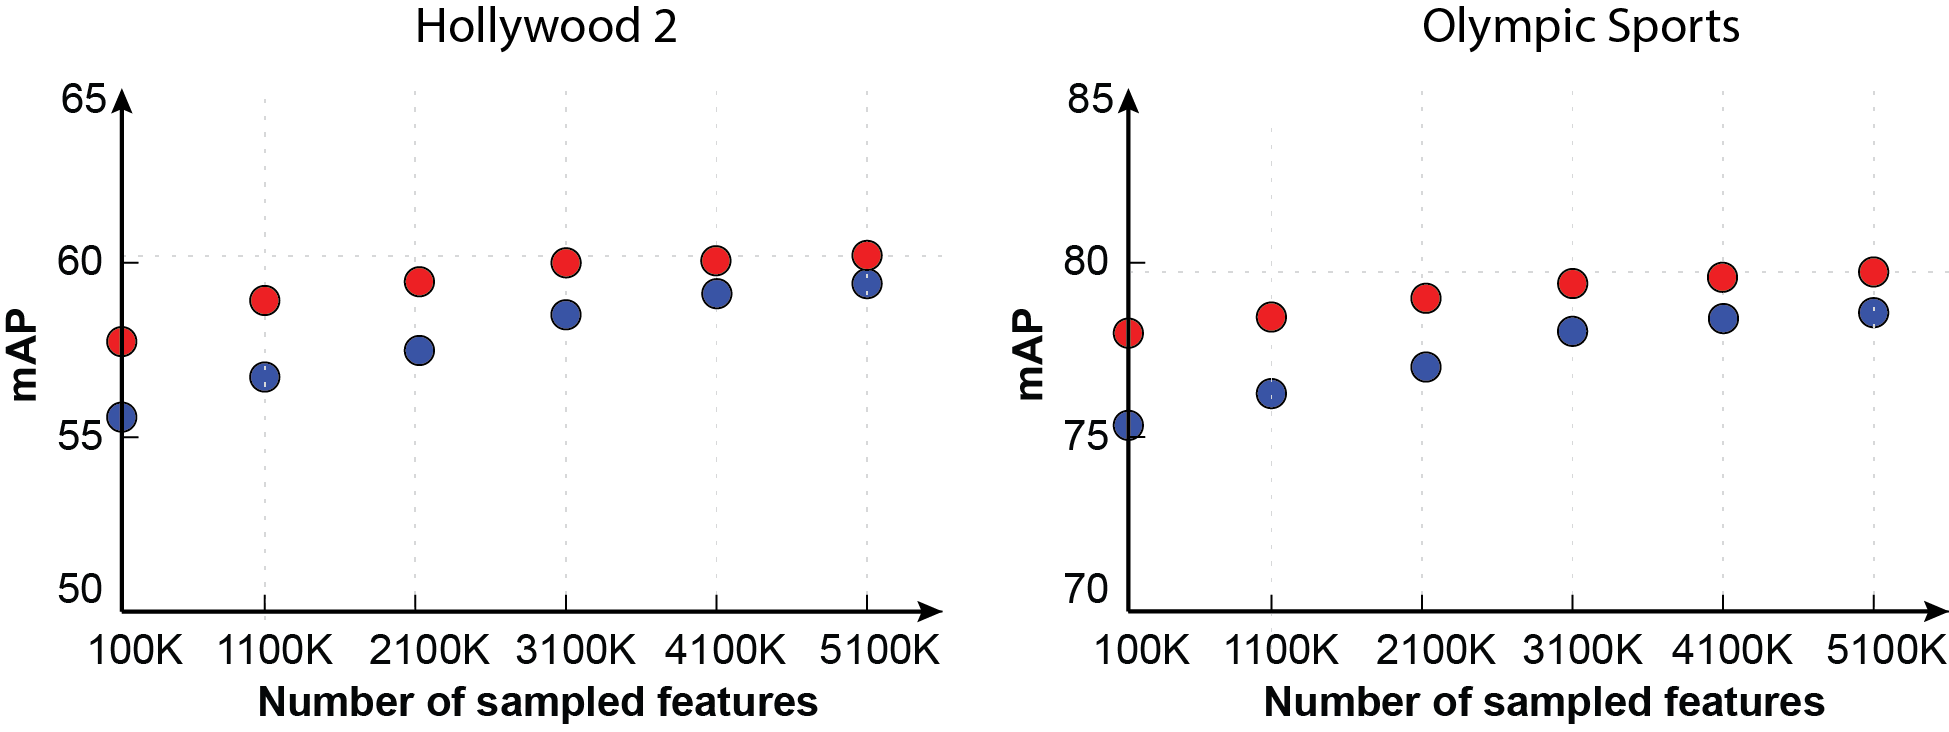
\includegraphics[width=0.98\linewidth]{fig/sampling.png}
\end{center}
\caption{Effect of feature sub-sampling when generating codebook.}
\label{fig:feature_sampling}
\end{figure*}
%%%%%%%%%%%%%%%%%%%%%%%%%%%%%%%%%%%%%%%%%%%%%%%%%%%%%%%%%%%%%%%%

%%%%%%%%%%%%%%% Table: Frameworks comparison %%%%%%%%%%%%%%%%%%%
\begin{table*}[h!]
\caption{Comparison of adopted frameworks for action recognition.}
\begin{center}
{
\begin{tabular}{ l| c c c c c }
\hline
Representation $\downarrow$ & Codebook & Encoding & Normalization & Classifier \\
\hline
Bag of Features & \textit{k}-means & VQ & L2 & MCSVM \\
Fisher vectors & GMM & Fisher vectors & L2+PW+IN & LSVM \\
\hline
\end{tabular}
}
\end{center}
\label{tab:frameworks}
\end{table*}
%%%%%%%%%%%%%%%%%%%%%%%%%%%%%%%%%%%%%%%%%%%%%%%%%%%%%%%%%%%%%%%%

\subsection{Impact of contextual features}
We conduct further experiments to measure the  contribution of our contextual features. Our Baseline corresponds to using only Foreground features for describing actions. Per-descriptor performances are compared to that established baseline. Also, we investigate the effect of combining contextual features with Foreground cues. As well, contextual features performance is evaluated under two action recognition representations \ie Bag of Features and Fisher vectors. Below, we present an analysis of obtained results.\\\\
\textbf{Representation}. As suggested in recent works \cite{perronnin2010, wang2013, xwang2013} Fisher vectors provides a boosted performance compared to traditional Bag of Feature representations. We found in our experiments that Fisher vectors also boost our contextual descriptors performance, as presented in Table \ref{tab:features}. However, we note that using Fisher vectors is less important with our CamMotion descriptor due to its low dimensionality. Even so, Fisher vectors are used for following analysis.\\\\
\textbf{Foreground-background}. As described in Section \ref{scene}, we perform a weak separation between background and foreground feature points. We measure the effect on performance of this separation in our contextual features. We note that this type of weak segmentation provides a significant boost in performance, as observed in Table \ref{tab:segmentation}. When feature points are localized on the background, SIFT features focuses on the scene appearance avoiding information of actors and foreground objects. The gain over computing SIFT over all features points is as follow: +0.3\% for HMDB51, +4.2\% for Hollywood2, +5.2\% for Olympics and +3.9\% for UCF50. The same behavior is observed with our CamMotion descriptor. Performance is boosted in all datasets when Fundamental Matrix is computed based on background tracks.\\\\
\textbf{Context appearance}. While by itself SIFT achieves a discrete performance, it produces notable improvements when combined with foreground descriptors. As Table \ref{tab:features} reports, performance is significantly improved over all datasets. Interestingly, we note that SIFT descriptor produces higher improvements in HMDB51 and UCF50 \ie +2.7\% and +2.4\% respectively.\\\\
\textbf{Camera motion}. Experiment results evidences that action recognition is noticeably improved when a global motion is incorporated to Foreground features. Our CamMotion provides slightly lower contributions in performance than the SIFT descriptor. We observe a significantly contribution over all datasets except on HMDB51 where recognition performance decrease. We attribute this negative effect to that HMDB51 presents several videos containing a shaking camera motion over all classes. This unable our CamMotion to capture discriminative cues over action categories. 

%%%%%%%%%%%%% Table: Effect of selected points %%%%%%%%%%%%%
\begin{table*}
\caption{Effect of separating background feature points on contextual features. Experimental results consistently show that contextual features are better captured on background regions. As observed, SIFT and CamMotion descriptors tend to be more 
discriminative when they are extracted from non-foreground feature points.}
\begin{center}
{
\begin{tabular}{|c|c c|c c c c|}
\hline
& \multicolumn{2}{|c|}{Feature points} & \multicolumn{4}{|c|}{Datasets} \\
Feature $\downarrow$ & Foreground & Background & HMDB51 & Hollywood2 & Olympics & UCF50 \\
\hline
SIFT & \checkmark & & 19.5\% & 22.1\% & 33.5\% & 44.7\% \\
SIFT & & \checkmark & \textbf{20.1\%} & \textbf{28.5\%} & \textbf{39.6\%} & \textbf{49.8\%} \\
SIFT & \checkmark & \checkmark & 19.8\% & 24.3\% & 34.4\% & 45.9\% \\
\hline
CamMotion & \checkmark & & 9.7\% & 14.9\% & 19.5\% & 13.7\% \\
CamMotion & & \checkmark & \textbf{14.1\%} & \textbf{22.1\%} & \textbf{27.2\%} & \textbf{19.5\%} \\
CamMotion & \checkmark & \checkmark & 12.9\% & 18.7\% & 21.8\% & 17.2\% \\
\hline
\end{tabular}
}
\end{center}
\label{tab:segmentation}
\end{table*}
%%%%%%%%%%%%%%%%%%%%%%%%%%%%%%%%%%%%%%%%%%%%%%%%%%%%%%%%%%%%

%%%%%%%%%%%%%% Table: Feature analysis %%%%%%%%%%%%%%%%%%%%%
\begin{table*}
\caption{Impact of our contextual features in recognition performance. Bag of Features generally performs poor than Fisher vectors. Both SIFT and CamMotion show important improvements in performance when they are combined with foreground descriptors.}
\begin{center}
{
\def\arraystretch{1.11}
\setlength{\tabcolsep}{3.66pt}
\begin{tabular}{ |c c c|c c c c| }
\hline
\multicolumn{3}{|c|}{Features} & \multicolumn{4}{|c|}{Datasets} \\
Foreground & SIFT & CamMotion & HMDB51 & Hollywood2 & Olympics & UCF50 \\
\hline
\multicolumn{7}{|c|}{Framework: Bag of Features} \\
\hline
\checkmark & & & 51.2\% & 60.1\% & 79.8\% & 85.9\% \\
& \checkmark & & 19.5\% & 28.7\% & 36.4\% & 45.7\% \\
& & \checkmark & 13.5\% & 21.8\% & 26.9\% & 19.3\% \\
\checkmark & \checkmark & & 53.8\% & 60.9\% & 81.1\% & 87.2\% \\
\checkmark &  & \checkmark & 50.9\% & 60.4\% & 80.6\% & 86.8\% \\
& \checkmark & \checkmark & 20.7\% & 36.2\% & 43.7\% & 50.3\% \\
\checkmark & \checkmark & \checkmark & 51.7\% & 61.6\% & 81.7\% & 87.6\% \\
\hline
\multicolumn{7}{|c|}{Framework: Fisher vectors} \\
\hline
\checkmark & & & 56.5\% & 62.4\% & 90.4\% & 90.9\% \\
& \checkmark & & 20.1\% & 28.5\% & 39.6\% & 49.8\% \\
& & \checkmark & 14.1\% & 22.1\% & 27.2\% & 19.5\% \\
\checkmark & \checkmark & & \textbf{59.2\%} & \textbf{63.5\%} & \textbf{91.6\%} & \textbf{93.3\%} \\
\checkmark &  & \checkmark & 55.9\% & 62.9\% & 91.3\% & 93.1\% \\
& \checkmark & \checkmark & 22.3\% & 36.5\% & 46.5\% & 54.3\% \\
\checkmark & \checkmark & \checkmark & \textbf{57.9\%} & \textbf{64.1\%} & \textbf{92.5\%} & \textbf{93.8\%} \\
\hline
\end{tabular}
}
\end{center}
\label{tab:features}
\end{table*}
%%%%%%%%%%%%%%%%%%%%%%%%%%%%%%%%%%%%%%%%%%%%%%%%%%%%%%%%%%%%%


\subsection{Comparison with the state of the art}
We set side by side our method with recent methods that address the same application using similar representations, \ie methods that use dense trajectory points to represent video sequences \cite{wang2013, jiang2012, jain2013} in Table \ref{tab:stateofart}. We also present results for our own implementation of \cite{wang2013}, which correspond to our baseline (Foreground). The gain over the recent paper \cite{wang2013}, which reports the best performance in the literature, is as follow: \textbf{+2\%} for HMDB51, \textbf{+1.4\%} for Olympic Sports and \textbf{2.6\%} for UCF50. We also achieve a comparable performance on Hollywood2 dataset with only 0.2\% less in the mAP value. Since Human Detection (HD) is not included in our trajectory extraction stage, a more direct comparison its the non-HD approach of Wang \etal \cite{wang2013}. In that case, our method outperforms their improved trajectories in \textbf{3.3\%} for HMDB51, \textbf{1.1\%} for Hollywood2, \textbf{2.3\%} for Olympic Sports and \textbf{3.3\%} for UCF50.

%%%%%%%%%%%%%% Table: State-of-the-art %%%%%%%%%%%%%%%%%%%%%%
\begin{table*}
\caption{Comparison with the state-of-the-art on challenging datasets. Our method improves reported results in the state-of-the-art for three different datasets, HMDB51, Olympic Sports and UCF50 and obtains competitive peformance in Hollywod2.}
\begin{center}
{
\begin{tabular}{ |l| c c c c| }
\hline
Approach $\downarrow$ & HMDB51 & Hollywood2 & Olympics & UCF50 \\
\hline
Jiang \etal \cite{jiang2012} & 40.7\% & 59.5\% & 80.6 & - \\
Jain \etal \cite{jain2013} & 52.1\% & 62.5\% & 83.2 & - \\
Wang \etal \cite{wang2013} non-HD & 55.9\% & 63.0\% & 90.2\% & 90.5\% \\
Wang \etal \cite{wang2013} HD & 57.2\% & \textbf{64.3\%} & 91.1\% & 91.2\% \\
\hline
\multicolumn{5}{|c|}{\textit{Our methods with Fisher vectors}} \\
\hline
Baseline (Foreground) & 56.5\% & 62.4\% & 90.4\% & 90.9\% \\
Foreground + SIFT & \textbf{59.2\%} & 63.5\% & \textbf{91.6\%} & \textbf{93.3\%} \\
Foreground + SIFT + CamMotion  & \textbf{57.9\%} & \textbf{64.1\%} & \textbf{92.5\%} & \textbf{93.8\%} \\
\hline
\end{tabular}
}
\end{center}
\label{tab:stateofart}
\end{table*}
%%%%%%%%%%%%%%%%%%%%%%%%%%%%%%%%%%%%%%%%%%%%%%%%%%%%%%%%%%%%%
